\documentclass[10pt,final,a4paper,oneside,onecolumn]{article}

%%==========================================================================
%% Packages
%%==========================================================================
\usepackage[a4paper,left=3.5cm,right=3.5cm,top=3cm,bottom=3cm]{geometry} %% change page layout; remove for IEEE paper format
\usepackage[T1]{fontenc}                        %% output font encoding for international characters (e.g., accented)
\usepackage[cmex10]{amsmath}                    %% math typesetting; consider using the [cmex10] option
\usepackage{amssymb}                            %% special (symbol) fonts for math typesetting
\usepackage{amsthm}                             %% theorem styles
\usepackage{dsfont}                             %% double stroke roman fonts: the real numbers R: $\mathds{R}$
\usepackage{mathrsfs}                           %% formal script fonts: the Laplace transform L: $\mathscr{L}$
\usepackage[pdftex]{graphicx}                   %% graphics control; use dvips for TeXify; use pdftex for PDFTeXify
\usepackage{array}                              %% array functionality (array, tabular)
\usepackage{upgreek}                            %% upright Greek letters; add the prefix 'up', e.g. \upphi
\usepackage{stfloats}                           %% improved handling of floats
\usepackage{multirow}                           %% cells spanning multiple rows in tables
%\usepackage{subfigure}                         %% subfigures and corresponding captions (for use with IEEEconf.cls)
\usepackage{subfig}                             %% subfigures (IEEEtran.cls: set caption=false)
\usepackage{fancyhdr}                           %% page headers and footers
\usepackage[official,left]{eurosym}             %% the euro symbol; command: \euro
\usepackage{appendix}                           %% appendix layout
\usepackage{xspace}                             %% add space after macro depending on context
\usepackage{verbatim}                           %% provides the comment environment
\usepackage[dutch,USenglish]{babel}             %% language support
\usepackage{wrapfig}                            %% wrapping text around figures
\usepackage{longtable}                          %% tables spanning multiple pages
\usepackage{pgfplots}                           %% support for TikZ figures (Matlab/Python)
\pgfplotsset{compat=1.14}						%% Run in backwards compatibility mode
\usepackage[breaklinks=true,hidelinks,          %% implement hyperlinks (dvips yields minor problems with breaklinks;
bookmarksnumbered=true]{hyperref}   %% IEEEtran: set bookmarks=false)
%\usepackage[hyphenbreaks]{breakurl}            %% allow line breaks in URLs (don't use with PDFTeX)
\usepackage[final]{pdfpages}                    %% Include other pdfs
\usepackage[capitalize]{cleveref}				%% Referensing to figures, equations, etc.
\usepackage{units}								%% Appropriate behavior of units
\usepackage[utf8]{inputenc}   				 	%% utf8 support (required for biblatex)
\usepackage{csquotes}							%% Quoted texts are typeset according to rules of main language
%\usepackage[style=ieee,doi=false,isbn=false,url=false,date=year,minbibnames=15,maxbibnames=15,backend=biber]{biblatex}
%\renewcommand*{\bibfont}{\footnotesize}		%% Use this for papers
%\setlength{\biblabelsep}{\labelsep}
%\bibliography{../../bib}

%%==========================================================================
%% Define reference stuff
%%==========================================================================
\crefname{figure}{Figure}{Figures}
\crefname{equation}{}{}

%%==========================================================================
%% Define header/title stuff
%%==========================================================================
\newcommand{\progressreportnumber}{25}
\renewcommand{\author}{Erwin de Gelder}
\renewcommand{\date}{December 9, 2019}
\renewcommand{\title}{Performance assessment of automated vehicles using real-world driving scenarios}

%%==========================================================================
%% Fancy headers and footers
%%==========================================================================
\pagestyle{fancy}                                       %% set page style
\fancyhf{}                                              %% clear all header & footer fields
\fancyhead[L]{Progress report \progressreportnumber}    %% define headers (LE: left field/even pages, etc.)
\fancyhead[R]{\author, \date}                           %% similar
\fancyfoot[C]{\thepage}                                 %% define footer

\begin{document}
	
\begin{center}
	\begin{tabular}{c}
		\title \\ \\
		\textbf{\huge Progress report \progressreportnumber} \\ \\
		\author \\ 
		\date
	\end{tabular}
\end{center}

\section{Previous meeting minutes}

\begin{itemize}
	\item I received feedback on an abstract for FISITA 2020. The paper we want to submit to FISITA 2020 describes a framework for the safety assessment of an autonomous vehicle.
\end{itemize}

\section{Summary of work}

\begin{itemize}
	\item I submitted the revised version of the ontology paper (Transportation Research Part C: Emerging Technologies). If this round of feedback takes as long as the previous round, I will get a decision near the end of 2019.
	\item I updated the abstract for FISITA 2020 based on the feedback I received during the previous meeting. In the corresponding paper, I want to propose a framework for the safety assessment of an autonomous vehicle using real-world scenarios.
	\item I continued my work on mining scenarios from real-world data. I want to write a conference paper on this subject for the Intelligent Vehicle Symposium (deadline: January 30, 2020). The approach can be roughly divided into two steps:
	\begin{enumerate}
		\item Describing the \emph{tags} related to the ego vehicle, actors (other than the ego vehicle), and the static environment. In this paper, the \emph{tags} focus on the activities of the ego vehicle and other actors, such as ``accelerating'' and ``changing lane left'', and the relative position of actors with respect to the ego vehicle, such as ``left of ego vehicle'' and ``in front of ego vehicle''.
		\item Mining the scenarios based on the \emph{tags}. To do this, the \emph{tags} are clustered into so-called n-grams, where each actor has its own n-gram. For example, a cut-in happens when one actor is first ``changing lane'' and then driving ``in front of ego vehicle''. At the same time, the ego vehicle should be ``following lane''.
	\end{enumerate}	
	While going through the code that is already available, I discovered some flaws. Fixing these flaws took me more time than expected, which is why the progress with the paper is not huge. I attached to this report what I have so far.
\end{itemize}

\section{Future plans}

In \cref{fig:planning}, the planning for my PhD is shown. Currently, there are three topics that I am working on:
\begin{itemize}
	\item \emph{Ontology}: I am waiting on a decision for the the revised manuscript.
	\item \emph{Overall methodology}: I am waiting for the decision based on the abstract.
	\item \emph{Scenario risk quantification}: Before writing a journal article on this subject, I want to publish a conference paper on scenario mining. Because of the deadline on the 30th of January, 2020, I want to have a first draft of the paper ready at the next progress meeting.
\end{itemize}

\begin{figure}[t]
	\centering
	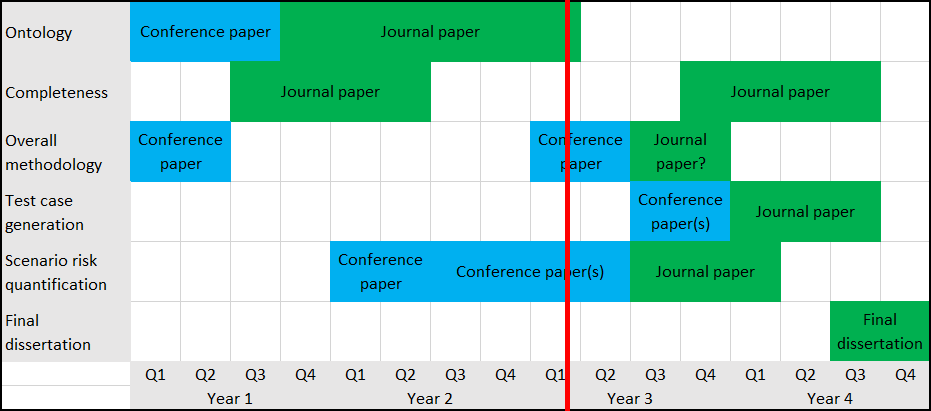
\includegraphics[width=\linewidth]{planning.png}
	\caption{Proposed planning at the time of this report. The red line indicated the time when writing this report. The planning is the same as the planning presented in the 23rd progress report.}
	\label{fig:planning}
\end{figure}



%\printbibliography

\clearpage
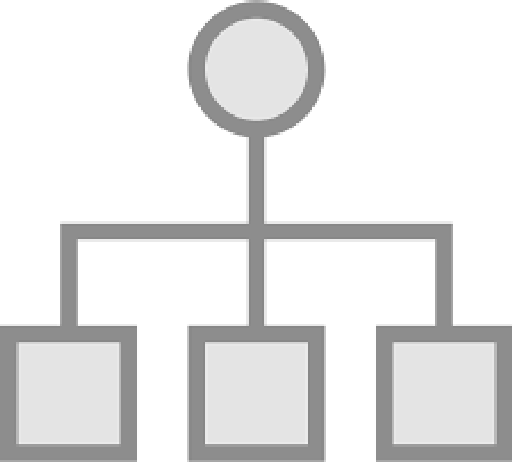
\includepdf[pages=-,pagecommand={},width=\paperwidth]{../../"20191010 Scenario Mining"/scenario_mining.pdf}

\end{document}